\documentclass[a4paper]{article}
\usepackage{graphicx}

\author{Steven Bronsveld\\Wouter Damen\\Kirsten Hagenaars\\Bram Pulles}
\title{\textbf{Heat Diffusion: openMP and MPI}}

\begin{document}
\maketitle

\tableofcontents

\pagebreak
\section{Hardware and software}
Table \ref{tab: hardware} shows the hardware specifications of the CPU from the computer that is used for getting test results. The computer further has 16 GB of ram and is running Arch Linux with kernel version 5.6.15-arch1-1. All of the programs are compiled with gcc version 10.1.0 and the following compiler flags: \texttt{-Wall -Wextra -Werror -pedantic -O3}.
\begin{table}[h]
    \centering
    \begin{tabular}{|l|l|}
        \hline
        Architecture:        &    x86\_64\\\hline
        CPU op-mode(s):      &    32-bit, 64-bit\\\hline
        Byte Order:          &    Little Endian\\\hline
        Address sizes:       &    39 bits physical, 48 bits virtual\\\hline
        CPU(s):              &    8\\\hline
        On-line CPU(s) list: &    0-7\\ \hline
        Thread(s) per core:  &    2\\\hline
        Core(s) per socket:  &    4\\\hline
        Socket(s):           &    1\\\hline
        NUMA node(s):        &    1\\\hline
        Vendor ID:           &    GenuineIntel\\\hline
        CPU family:          &    6\\\hline
        Model:               &    94\\\hline
        Model name:          &    Intel(R) Core(TM) i7-6700HQ CPU @ 2.60GHz\\\hline
        Stepping:            &    3\\\hline
        CPU MHz:             &    1200.022\\\hline
        CPU max MHz:         &    3500.0000\\\hline
        CPU min MHz:         &    800.0000\\\hline
        BogoMIPS:            &    5202.65\\\hline
        Virtualization:      &    VT-x\\\hline
        L1d cache:           &    128 KiB\\\hline
        L1i cache:           &    128 KiB\\\hline
        L2 cache:            &    1 MiB\\\hline
        L3 cache:            &    6 MiB\\\hline
        NUMA node0 CPU(s):   &    0-7\\
        \hline
    \end{tabular}
    \caption{Hardware specifications.}
    \label{tab: hardware}
\end{table}

\section{Testing}
In order to gather performance information we use a tester made by one of the team members. The tester is written in Bash and supports a wide variety of options, including: minimum and maximum N and rank over which will be iterated, the epsilon value, the initial heat value, a timeout, the number of iterations to run, and the suite which we want to test (MPI, openMP, sequential or any combination of these). It further has a verbosity which can be set so we can produce human readable output or output in the CSV format so it is easy to process the test data and make graphs from them.

Lastly, we used a seperate Bash script to call the tester on a wide variety of configurations which automatically runs all of them, post processes the CSV output further and puts the results in seperate files, this way we could run tests for hours without having to do anything manually.

% TODO Explain what split join and zero means

\section{Sequential}
\textit{Unless stated otherwise, runtimes shown in figures have been acquired using $\texttt{N} = 1000000$, $\texttt{eps} = 0.01$ and $\texttt{HEAT} = 100$. Furthermore, every version was executed $20$ times and each individual run is shown by a dot in the figure.}\\

\noindent We have added a check for malloc failure to the program. After running valgrind on the program, which alerted us to the memory leak that was left by the heap-allocated vectors, we also added the freeing of the allocated memory at the end of the program.

We have also implemented the option of passing the values for N, EPS and HEAT as command-line arguments to the program, which allows us to test more easily and automatically. Parsing of the arguments is not included in the runtimes.

Since we came up with multiple possible improvements to the program, we decided to make multiple versions and compare these. Here is a list of these versions and how they differ from the original program (aside from what is mentioned above). Note that the openMP and the MPI versions use the same naming conventions.
\begin{itemize}
    \item
        In the \textit{split} version, the relaxation step and the stability check are done in separate loops. The stability check terminates once some \texttt{i} for which \texttt{(fabs(out[i] - in[i]) > eps)} holds is found.
    \item
        In the \textit{split\_zero} version, the relaxation step and the stability check are done in separate loops and the stability check is terminated early in the same way as this is done in \textit{split}. Since the array resulting of the relaxation ends with some amount of zero's (possibly none) and we know where those zero's will start, we terminate the loop just before arriving at the zero's.
    \item
        In the \textit{join} version, the relaxation step and stability check are combined into one loop. A variable \texttt{stable} is kept which is returned at the end to signify if the new array is stable. The \texttt{stable} variable is updated during every iteration of the relaxation for loop if it is not already declared unstable, \texttt{if (stable) stable = fabs(out[i] - in[i]) > eps}.
    \item
        In the \textit{join\_zero} version, the relaxation step and stability check are combined into one loop just like the \textit{join} version. Similarly to \textit{split\_zero}, the loop terminates early since we know from which point on the remainder of the array is all zero's.
\end{itemize}

% TODO Add a figure with increasing N on the x axis and time on the y axis, map the different runtimes of the sequential algorithms as lines through the average runtime of a specific N (with an optional error bar on the average points (probably won't look good because the error bars will overlap)), the different algorithms are represented with different lines having different colors. This figure will show that the zero's versions do not slow down when N increases.

% TODO Add a figure with the heat value on the x axis and time on the y axis, we choose a fixed N and eps, e.g. N = 100000 and eps = 0.01. The rest of the figure is analogous to the figure described above, so with different colored lines (one for each version) going through the average runtimes for the different heat values. This figure will show that the advantage of the zero's versions is not really present when heat and eps increase.

\section{OpenMP}
For the openMP versions of the program, we have used \texttt{\#pragma omp parallel for schedule(...)} for the loops in the functions \texttt{init} and \texttt{relaxAndStable}. To find out which scheduling strategy performes the best, we have made a comparison between the scheduling strategies. The results are shown in the following figure, note that the dynamic scheduling strategy is not included since it often took more than $10$ seconds, making it way slower than the others.

% Add a figure for N and heat on the scheduling strategies.
% 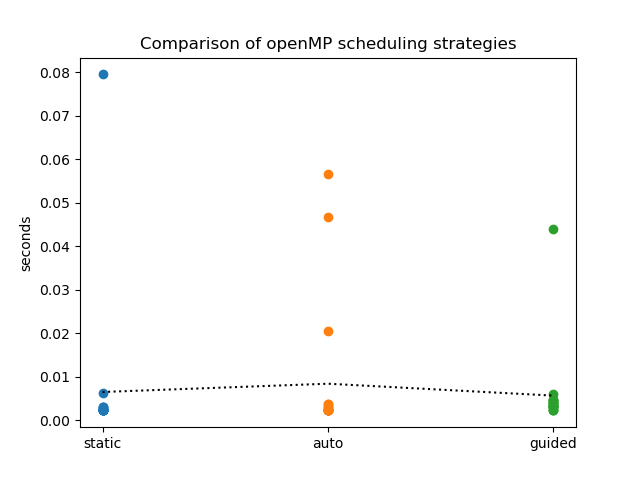
\includegraphics[scale = 0.5]{graphs/Comparison of openMP scheduling strategies.png}

This may not be clearly visible from the figure, but we found that the static scheduling strategy leads to the smallest runtimes on average. Therefore we have used this stategy for the final openMP versions.

We have also tried out if using openMP's reduction decreases runtimes. We found that this is not a good approach, because we want to stop searching once we find one instance of \texttt{fabs(out[i] - in[i]) <= eps} being false, which does not happen when using \texttt{ reduction(\&\&: stable)}. Using openMP's support for for-loops in the \texttt{init} and \texttt{relaxAndStable} functions does achieve this. The difference between stopping early and using reduction is depicted in the figure below.

% Add a figure for N and heat on reduction yes/no.
% 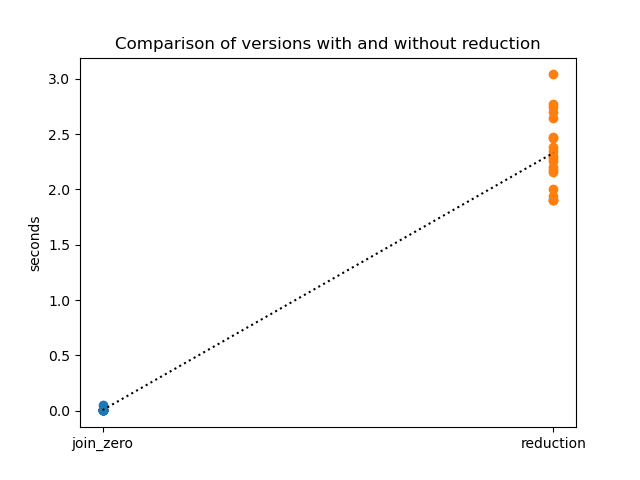
\includegraphics[scale = 0.5]{graphs/Comparison of versions with and without reduction.png}

As stated before, we have made multiple optimized sequential versions. We have applied the openMP's support for loops on all of these versions to see which performes best when openMP is used. The following figure shows the results.

% Add a figure for N and heat comparing the major versions.
% 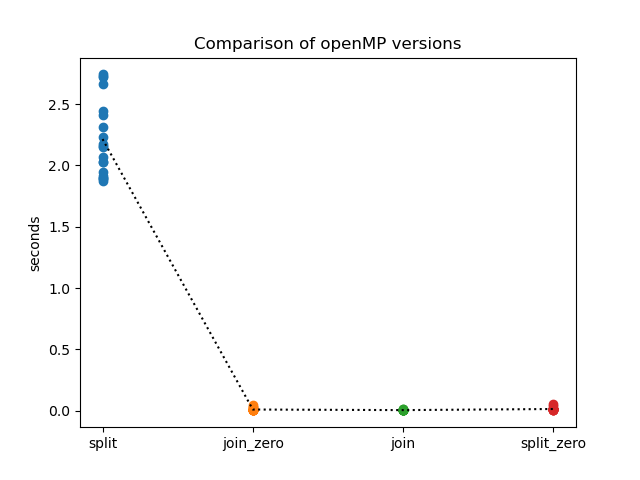
\includegraphics[scale = 0.5]{graphs/Comparison of openMP versions.png}

Surprisingly, even though the \textit{split} version performed faster in the sequential setting, the \textit{joined} version performs faster in openMP.

\section{MPI}
For MPI we compared the performance of versions in which we use \texttt{MPI\_Allgather}
and \texttt{MPI\_Allreduce} and of versions in which we manually communicate the results using \texttt{MPI\_Send} and \texttt{MPI\_Recv}. It was very apparent that using \texttt{MPI\_Allgather} for the heat array and \texttt{MPI\_Allreduce} for the stability boolean is much faster than manual messages. The reason for this, as discussed in the lectures,
is that the straightforward way to do manual messages causes one process to do all of the reduction work. Whereas the MPI reduction methods will automatically optimize the message structure to divide the reduction work across the processes as much as possible.

% TODO Finish this section and add two addition figures one with N on the x axis and one with heat on the x axis. (And also compare different numbers of ranks?)

\section{Performance}
We made a general observation regarding the size of the vector. Whenever we increase the vector size all of the non-zero versions become considerably slower, while the zero versions keep the same runtime, since they ignore a huge part of the vector, namely everything after the first zero. This optimization has a smaller impact when the heat value is increased or the epsilon value is decreased. Because in this case the zero versions have a big advantage at the start, when the heat is not diffused so far yet. However, the further the heat diffuses the smaller the advantage of the zero versions becomes. Thus, if the vector is relatively small the advantage of the zero versions is negligable.

The sequential algorithms are faster when split is used than when join is used. Because with split we can stop checking if the array is stable and return when we reached a point which is not below epsilon yet. With join we can stop computing the difference between the two arrays, however we still need to check if we already found a value which proves that the array is unstable. This means that join needs to do more work than the split versions, so the split versions are faster than the join versions.

The openMP algorithms are faster when join is used than when split is used. Because join can easily be run in parallel, since all the results are gathered into one \texttt{stable} variable which is returned at the end. But when using split checking if the array is stable cannot be run in parallel, since the for loop stops/returns whenever an unstable cell in the array is found. This means that the split version slows the openMP algorithms down a lot due to the sequential nature of the \texttt{isStable} function. So for openMP the join versions are way faster than the split versions.

% TODO MPI conclusions

\section{Task division}
Here we give an overview of the task division between the members of our group.
\begin{itemize}
    \item \textbf{Steven Bronsveld and Wouter Damen} worked on the MPI code. They first planned out what optimizations where possible, and what different MPI-techniques where. Then they devided the work such that Wouter made the programm using the different forms of gather, and Steven used MPI-messages.
    \item \textbf{Kirsten Hagenaars and Bram Pulles} worked on the openMP code. Bram further made the testing setup, the Bash scripts, and the Makefiles to compile all of the code. Kirsten additionally made all of the plots in this report using Python.
    \item \textbf{All}: We frequently met each other online to discuss our findings and the progress we made on the project. Each one of us wrote the section in the report corresponding to the code on which he/she has worked. We all worked on improving the sequential version before we splitted into two groups and dived into openMP and MPI seperately. The decision to split into pairs was made to reduce the overhead of communication when working on the individual sections. We also shared ideas for optimizations and gave each other mental support.
\end{itemize}

\end{document}
